% =============================== 5. Q2 ===============================
\section{Question 2: Optimal Repositioning on a Typical Day}\label{sec:q2}

\begin{figure}[htbp]
\centering
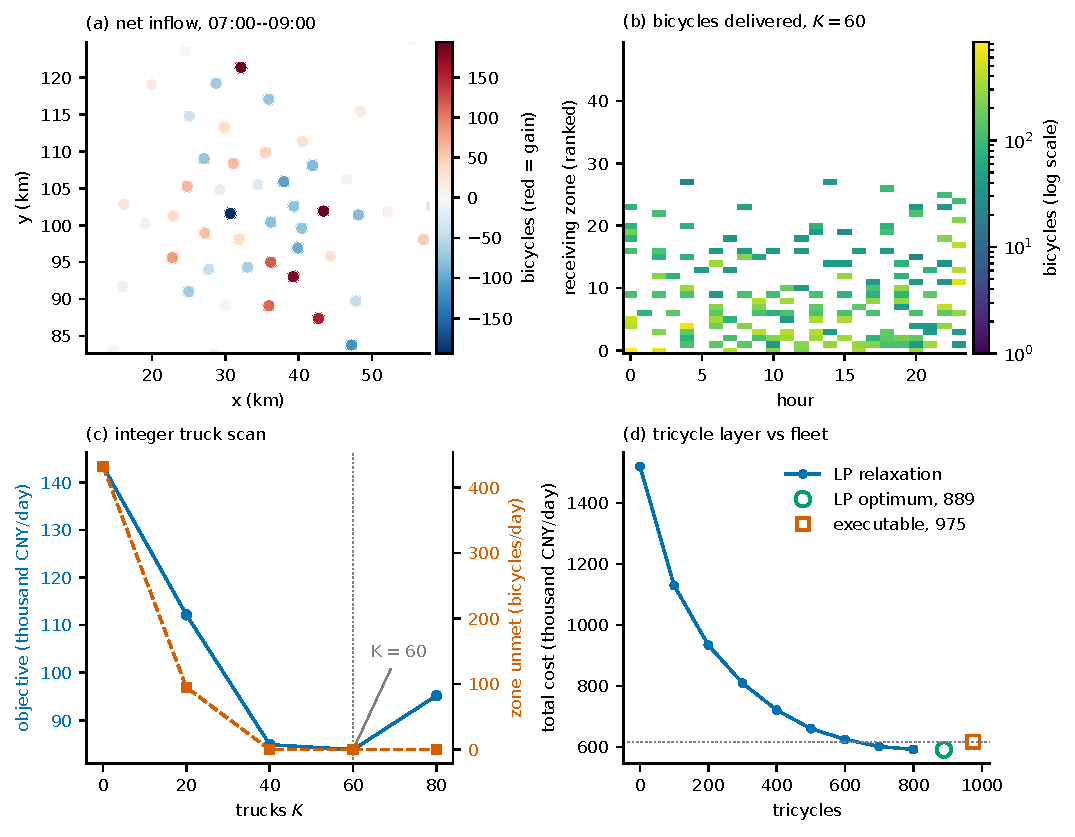
\includegraphics[width=0.9\linewidth]{../figs/fig4_q2.pdf}
\caption[Q2: flow, truck schedule, fleet scans]{Q2. (a) Net flow in the morning peak
by zone: the core gains bicycles, the residential periphery loses them. (b) The
$K=60$ truck schedule: bicycles delivered by hour and receiving zone, from the
integer plan. (c) Integer objective and zone unmet against the truck fleet; $K=60$
is the minimum of the compared grid. (d) Total cost against fleet size from the joint
conserving replay, scaling the executable allocation by 0.70--1.30; the square marks
the 1,233-tricycle executable plan.}
\label{fig:q2}
\end{figure}

\subsection{Two scales of imbalance}

At the
50-zone scale, the flow-only inventory path of each zone,
\begin{equation}
\tilde I_{zt} \;=\; I_{z0} + \sum_{s\le t}\left(a_{zs}-d_{zs}\right),
\label{eq:path}
\end{equation}
never reaches zero from the initial-inventory proxy of 343,638 bicycles; $a$ and
$d$ are the hourly arrivals and departures of a typical day scaled by $1/p$. At that
scale the 50-zone program with no dispatch ($K=0$ in \tabref{tab:q2scan}) leaves
432.23 departures unserved, 0.02\% of 2,132,542.

\textbf{That number is an aggregation artefact.} The same scaled flows and the same
343,638-bicycle inventory, replayed at cell resolution with a conserving process
(departures Poisson,
arrivals generated by served departures, the city total fixed at 343,638 at every
step), leave \textbf{17.40\%} of departures unserved with \emph{no repositioning at
all} (371,129.50 of 2,132,542.19) and \textbf{17.31\%} with the $K=60$ truck plan
running (369,181.08). A zone-level average hides the cell-level shortfall because
cells with opposite imbalances cancel inside a zone. Every statement about service in
this paper is therefore made at cell resolution; the zone model is used only to
\emph{schedule trucks}, which is what it is good for.

\textbf{The truck plan is a balance instrument, not a service instrument.} Running the
$K=60$ plan in the conserving replay removes 1,948 departures (371,129.50 $\to$
369,181.08) for 83,807.74 CNY/day, 43.01 CNY per departure removed against a 6 CNY
service penalty: the trucks pay for end-of-day balance and for nothing else. That is
why the tricycle layer, which can see inside a zone, does the service work.

Rebalancing is therefore not a rescue operation; it is a \emph{reset}, in two layers:
trucks move bicycles between zones, tricycles between cells inside one zone. They are
optimised in that order, because a tricycle cannot undo a zone-level shortage.

\subsection{The truck layer: a time-space network program}

Let $z=1,\dots,50$ index zones and $t=0,\dots,23$ hours. The decision variables are
the inventory $I_{zt}$, the bicycles moved $x_{ijt}$ and the trucks moved $m_{ijt}$ on
arc $(i,j)$ of a sparse zone graph (the eight nearest neighbours of each zone within
9 km; 290 arcs, mean length 5.97 km), the trucks present $n_{zt}$, the unmet
departures $u_{zt}$, and the end-of-day deviations $dp_z,dm_z$.

{\allowdisplaybreaks
\begin{align}
\min\quad
& c_{\text{km}}\sum_{t}\sum_{(i,j)} d_{ij}\,m_{ijt}
+ c_{\text{load}}\sum_t\sum_{(i,j)} x_{ijt}
+ w\sum_t\sum_z u_{zt}
+ c_{\text{dev}}\sum_z\left(dp_z+dm_z\right)
+ f K \label{eq:q2obj}\\
\text{s.t.}\quad
& I_{z,0} = I_{z0}, \label{eq:q2init}\\
& I_{z,t+1} = I_{z,t} + a_{zt} - \left(d_{zt}-u_{zt}\right)
  - \sum_{j} x_{zjt} + \sum_{i} x_{izt}, \label{eq:q2bal}\\
& \sum_j x_{zjt} + d_{zt} - u_{zt} \;\le\; I_{z,t}, \label{eq:q2serv}\\
& x_{ijt} \;\le\; Q\,m_{ijt}, \label{eq:q2cap}\\
& \sum_{j} m_{zjt} \;\le\; n_{zt}, \label{eq:q2truck}\\
& n_{z,t+1} = n_{zt} - \sum_j m_{zjt} + \sum_i m_{izt},
  \qquad \sum_z n_{z,0} = \sum_z n_{z,23} = K, \label{eq:q2fleet}\\
& \big[I_{z,23} + a_{z,23} - (d_{z,23}-u_{z,23})
   - \textstyle\sum_j x_{zj,23} + \sum_i x_{iz,23}\big] - I_{z0} = dp_z - dm_z,
  \label{eq:q2dev}\\
& I,u,dp,dm \ge 0,\qquad x,m,n \in \mathbb{Z}_{\ge 0}. \notag
\end{align}}

The objective prices five things. $c_{\text{km}}=6$ CNY per truck-kilometre is the
running cost; $c_{\text{load}}=0.5$ CNY per bicycle loaded and unloaded is handling;
$w=6$ CNY per unmet departure is a service penalty set above the cost of moving a
bicycle; $c_{\text{dev}}=3$ CNY per bicycle of end-of-day drift, linearised by $dp,dm$,
penalises leaving the system out of balance; and $f=600$ CNY per truck per day is the
ownership cost of a truck, charged on $K$.

The constraints are the physics. \eqnref{eq:q2bal} is conservation of bicycles;
\eqnref{eq:q2serv} is the event-order constraint: a truck may take away only bicycles
present at the start of the hour, before that hour's departures are served;
\eqnref{eq:q2cap} couples bikes to trucks ($Q=40$ bicycles per truck);
\eqnref{eq:q2truck}--\eqnref{eq:q2fleet} conserve the truck count, with $K$ at the
start and at the end of the day but no per-zone requirement; end-of-day positions are
matched to the start-of-day ones by the deadhead relocation reported below, outside the
objective; \eqnref{eq:q2dev} defines the end-of-day deviation that
makes the plan a reset. Bicycles, trucks and truck presence are integer variables; as
a continuous program it would be cheaper but would describe fractions of a
truck and of a bicycle.

The continuous LP plan, re-checked
on its own demand, violates the stock constraint in 3 of 1,200 zone-hours and would
take 717.54 bicycles out of zones that do not have them. The integer plan has zero
violations of every constraint: maximum load 40 bicycles, maximum trip 46.92 minutes
against the 60-minute hour, truck-conservation residual 0, at least 0.81 bicycles of
event-order slack in every zone-hour, and minimum inventory 1,891.36. The LP relaxation
at $K=60$ costs 82,968.0671 and the MILP 83,807.7438, a gap of 839.68 CNY (1.01\%). The plan also has an end-of-day deadhead of 1,023.76 truck-kilometres
(6,142.58 CNY), which is not in the objective and is reported separately; repeating the
daily plan requires it. The truck cost is common to both totals in the comparison, and
the deadhead enters neither: adding it to both sides would leave the absolute saving
unchanged but lower the percentage below the 65.38\% quoted.

\subsection{Trucks alone: the single-layer baseline}

\tabref{tab:q2scan} scans the integer fleet on the five grid points that were solved.
$K=0$ is the no-dispatch point; $K=60$ is the minimum of the compared grid and the
baseline against which the tricycle layer is evaluated, not the Q2 recommendation
once tricycles are available.

\begin{table}[htbp]
\centering
\footnotesize
\caption[Integer truck scan]{Integer truck plan by fleet size. ``Zone unmet'' is
the unmet departures of the 50-zone model, priced at 6 CNY; the objective includes the
fixed cost $600K$, the kilometre and loading costs, and the deviation. The LP relaxation
at $K=60$ costs 82,968.0671.}
\label{tab:q2scan}
\scriptsize
\begin{tabular}{@{}rrrrrr@{}}
\toprule
$K$ & \textbf{Moved} & \textbf{Truck-km} & \textbf{Zone unmet} & \textbf{Dev} &
\textbf{Objective} \\
\midrule
0  & 0      & 0.00     & 432.23 & 46,930.39 & 143,384.53 \\
20 & 9,503  & 1,767.02 & 95.01  & 28,083.10 & 112,172.98 \\
40 & 19,104 & 4,097.39 & 0      & 8,907.88  & 84,860.02 \\
\textbf{60} & \textbf{24,949} & \textbf{5,659.17} & \textbf{0} &
\textbf{459.41} & \textbf{83,807.74} \\
80 & 24,863 & 5,495.85 & 0      & 586.96    & 95,167.44 \\
\bottomrule
\end{tabular}
\end{table}

At $K=60$ the 24,949 relocated bicycles cost
5,659.17 truck-kilometres, and the end-of-day deviation falls from 46,930.39 at $K=0$
to 459.41: the objective is dominated by balance, not by service, because the zone
model has almost no unmet demand to remove. More trucks bring diminishing returns
after 60: $K=80$ adds 11,359.70 CNY and moves 86 fewer bicycles.

The hold-out replay fixes the plan on the five training days and replays it on the
two held-out days. On 12 May, at
0.9291 times the design volume, it leaves 704.74 departures unserved and ends
53,255.64 bicycles away from balance; on 19 May, at 1.1066 times the design volume, it
leaves 14,232.37 unserved, 0.60\% of that day's departures, and 51,718.20 away from
balance. No zone-hour hits the truck capacity in either replay. The service cost of a
volume surprise is small in percentage terms, but the end-of-day balance deteriorates
sharply: the plan is built for the typical day, not for the tail.

\subsection{The tricycle layer: replacing within-zone walking with a fleet}

The truck plan equalises zone totals. Inside a zone, riders can already borrow a
bicycle up to 300 m away, but the 300 m radius reaches no neighbour cell centre on this
grid, so walking cannot move a bicycle across a cell boundary. The tricycle layer is
therefore a within-zone transport problem. A tricycle carries $Q_{\text{tri}}=20$
bicycles, travels at 15 km/h, needs 0.5 minutes per bicycle handled, makes trips of at
most 5 km, and operates from 07:00 to 20:00. Its cost is 300 CNY per tricycle-day,
0.2 CNY per vehicle-kilometre ($c_{\text{km}}$), and the same 6 CNY penalty
($w_{\text{tri}}$) on any cell-level departure left unserved. The layer is solved zone
by zone; the truck layer is held fixed at the $K=60$ plan.

A deficit cell $a$ is paired with the 12 nearest
stock-holding cells $b$ inside the trip limit; $y_{ab}$ bicycles move from $b$ to $a$,
$u_a$ departures stay unserved, $e_a$ the departure still unmet after trucks and
walking, $I_b$ the donor stock at the hour start, $d_{ab}$ the distance,
$\nu_z$ the zone's tricycles, and $\theta_{ab}$ the tricycle-hours one bicycle on
arc $ab$ occupies: loaded leg out, empty return, one full load, plus handling at both
ends. For each zone-hour,
\begin{equation}
\begin{aligned}
&\min\;\sum_{ab}\frac{c_{\text{km}}}{Q_{\text{tri}}}\,d_{ab}\,y_{ab}
  +w_{\text{tri}}\sum_a u_a\\
&\text{s.t.}\;\;\sum_b y_{ab}+u_a=e_a,\qquad
\sum_a y_{ab}\le I_b,\qquad
\sum_{ab}\theta_{ab}\,y_{ab}\le\nu_z ,
\end{aligned}
\label{eq:q2tri}
\end{equation}
with flows and unmet non-negative. The LP solution is rounded to whole bicycles under
each donor's integer stock and split into trips of at most $Q_{\text{tri}}$. The fixed
list is assigned to the zone's tricycles by earliest finish inside the shift, and the
smallest integer fleet that places every trip replaces the fractional count zone by zone.

The joint conserving replay is optimised by coordinate descent over integer per-zone
fleets: each candidate changes one zone by $\pm1$ or $\pm2$ tricycles and is evaluated
by a full 24-hour simulation of the city, because a fleet change alters the served
departures and therefore every later arrival. From the scaled start (1,271 tricycles,
1.10 times the earlier allocation) the descent settles
at \textbf{1,196 tricycles}, a layer of 707,118.68 and a total of 790,926.43, with
57,759.37 cell-level departures unserved and 8,812.18 tricycle-kilometres. That
allocation is not yet executable: the per-zone trip schedule cannot always be run at the
fleet the descent evaluates, so each zone is raised to the smallest integer fleet at which
its schedule places every trip. The executable plan is \textbf{1,233 tricycles}, a layer
of \textbf{712,063.25} --- 369,900 fixed, 1,772.82 kilometre cost and 340,390.43 the 6 CNY
penalty on 56,731.74 unserved --- and a total of \textbf{795,870.99 CNY/day}, a saving of
\textbf{1,503,023.20 (65.38\%)} against the 2,298,894.20 no-tricycle baseline. The
executable fixed point costs 4,944.57 (0.62\%) more than the descent allocation and
serves 1,027.64 more departures; it is the plan we report.

The gap between the two allocations is the price of executability, and it is small. The
37 added tricycles cost 11,100 in fixed cost and 10.38 in kilometres, while the
1,027.64 departures they serve are worth 6,165.82 in penalty; the net is the
4,944.57 difference. The conserving replay values a tricycle more highly than the zone
model did, because it sees the cell-level shortfall that the zone totals cancel; the
6 CNY penalty is doing the work.

\subsection{The three schemes on their own calibers}

\tabref{tab:q2schemes} puts the schemes side by side. The two panels are
\emph{different accounting calibers}: the truck plan was optimised in the zone model,
where it removes all 432.23 unmet departures at $K=0$ and costs 83,807.74 at $K=60$;
the same plan, priced in the cell model, carries a cell deficit of 369,181.08 that the
zone model cannot see, and the two-tier plan is the only row that removes most of it.

\begin{table}[htbp]
\centering
\footnotesize
\caption[Q2 schemes]{Q2 schemes at two calibers. Panel A is the 50-zone model in which
the truck plan is optimised; Panel B is the cell-level conserving model, with the same
$K=60$ truck plan and the cell deficit priced at 6 CNY. ``Truck'' is the zone-level
truck objective, including its own zone penalty and deviation in Panel A; ``tricycle
operating'' is fixed, kilometre and handling cost; ``cell penalty'' is 6 CNY times the
cell-level unmet. The 2,298,894.20 baseline is the cell-level cost of the truck-only
plan, not the 83,807.74 zone-level objective.}
\label{tab:q2schemes}
\scriptsize
\begin{tabular}{@{}lrrrrr@{}}
\toprule
\textbf{Scheme} & \textbf{Fleet} & \textbf{Truck} & \textbf{Tricycle operating} &
\textbf{Cell penalty} & \textbf{Total} \\
\midrule
\multicolumn{6}{@{}l}{\emph{Panel A: zone-level caliber (unmet 432.23 at $K=0$, 0 at $K=60$)}}\\
No dispatch & $K=0$ & 143,384.53 & --- & --- & 143,384.53 \\
Trucks only & $K=60$ & 83,807.74 & --- & --- & 83,807.74 \\
\midrule
\multicolumn{6}{@{}l}{\emph{Panel B: cell-level caliber (cell unmet shown in the last column)}}\\
Trucks only & $K=60$ & 83,807.74 & --- & 2,215,086.45 & 2,298,894.20 \\
Two-tier & $K=60$, 1,233 tricycles & 83,807.74 & 371,672.82 & 340,390.43 &
\textbf{795,870.99} \\
\bottomrule
\end{tabular}

\smallskip
\raggedright Cell-level unmet: 369,181.08 for trucks only; \textbf{56,731.74} for the
two-tier plan.
\end{table}

Panel A gives the single-layer result: 143,384.53 at $K=0$ against 83,807.74 at $K=60$,
a saving of 59,576.79 (41.55\%). Panel B gives the two-tier result: 2,298,894.20
against 795,870.99, a saving of 1,503,023.20 (65.38\%). The two savings answer different
questions: 41.55\% is what trucks do for the zone model, 65.38\% what the tricycle
layer adds once the zone model's blind spot is priced, and neither is a system-level
claim.

\subsection{Uncertainty and the limits of the number}

The numbers above are a planning midpoint, not an expectation or a median. The joint
sample of Section~\ref{sec:sens} re-evaluates the executable allocation inside the
conserving replay at every draw, with the fleet held at its 1,233 tricycles, so the
interval describes the cost of the reported plan under parameter uncertainty, not the
cost of a re-optimised fleet. Across the 128 joint draws the two-tier total has
P5/P50/P95 \textbf{316,247 / 585,792 / 1,242,903} CNY/day, the executable unmet
1,178 / 14,322 / 111,974, and the saving share $-0.5757$ / 0.2458 / 0.7352. The 65.38\%
is therefore a midpoint: in 36 of the 128 draws the two-tier plan costs more than no
tricycles at all --- draws in which the fleet would be cut, not kept. The anchors are
small: the reference draw's truck objective is the LP's 82,968.07 rather than the integer
plan's 83,807.74, a shift of 839.67 on every draw, and the replay conserves the city
total to within 0.0004 of 343,638 in every draw.

Two boundaries follow. The 1,233-tricycle fleet is the smallest executable fixed point
of the descent allocation, not a global optimum: the coordinate descent is a local
search over integer fleets, and the joint curve of Figure~\ref{fig:q2}(d) is flat
around the optimum. And the intervals are fixed-fleet intervals --- every draw pays for
1,233 tricycles and the truck plan is re-solved on the draw's demand --- so a draw that
re-optimised the fleet would lie below them; they are an outer bound on the
uncertainty of the reported plan.
